% !TeX spellcheck = de_AT_frami

\section{Die mathematische Problemstellung}
Wir möchten das folgende mathematische Problem numerisch lösen:\\
\begin{center}
	\begin{tabular}{ll}
	\textbf{Input:} &Eine invertierbare Matrix $A\in \Rnn$ und ein Vektor $b\in \Rn$. ~\\
\textbf{Output:} &Der Vektor $x\in \Rn$, sodass
\end{tabular}
$$Ax = b.$$
\end{center}
Bemerkungen:
\begin{itemize}
	\item Da $A$ invertierbar ist, existiert für jede rechte Seite $b$ genau eine eindeutige Lösung $x = A^{-1}b$.
	\item Die Berechnung der inversen Matrix $A^{-1}$ ist sehr teuer (z.B. $n$ mal Lösen mit Einheitsvektoren) und wird in der Praxis stets vermieden, da man meist nur an $b \mapsto A^{-1}b$ interessiert ist.
\end{itemize}
Zur Lösung von linearen Gleichungssystemen gibt es im Wesentlichen zwei große Verfahrensklassen:
\begin{itemize}
	\item \textbf{Direkte Methoden:} Faktorisieren und Lösen
	\begin{itemize}
		\item Gauss Elimination und $LR$-Zerlegung, Cholesky Zerlegung
		\item Gram-Schmidt/Householder/Givens und $QR$-Zerlegung
		\item ...
	\end{itemize}
    $\rightarrow$ Gut geeignet für kleine Probleme ($n \leq 10^5$)\\
    $\rightarrow$ Bei großen Problemen: Zu langsam, Rundungsfehler, ...\\
    $\rightarrow$ direkt = endlich viele Schritte
	\item \textbf{Iterative Verfahren:}
	\begin{itemize}
		\item Krylov-Unterraum Verfahren
		\item Splitting-Verfahren (Fixpunktiteration)
		\begin{itemize}
			\item \textbf{Richardson}
			\item Jacobi
			\item Gauß-Seidel, SOR
		\end{itemize}
	\end{itemize}
	    $\rightarrow$ Brauchen i.d.R. nicht die Matrix selbst, sondern nur die Funktion $x \mapsto Ax$ (Matrix-Vektor Produkt)\\
$\rightarrow$ Gut geeignet für große (dünn-besetzte) Probleme ($n \geq 10^5$), wie sie häufig in Anwendungen vorkommen\\
$\rightarrow$ direkt $\neq$ iterative = indirekt = ggf. unendlich viele Schritte
\end{itemize}
%%
%%
\textbf{Der Ansatz für iterative Verfahren:}\\
Wir möchten eine Folge $(x^k)_k$ von Vektoren $x^k \in \Rn$ konstruieren, sodass die folgenden Eigenschaften erfüllt sind.
\begin{itemize}
	\item Die Folge $(x^k)_k$ konvergiert.
	\item Der Grenzwert $x^*$ löst die Gleichung: $Ax^* =b$.
\end{itemize}
Ausgehend von einem (i.d.R. beliebigen) Startvektor $x^0 \in \Rn$ berechnen wir Schritte $p^k\in \Rn$ mit der Absicht, dass wir uns durch die Iterationsvorschrift
$$x^{k+1} = x^k + p^k $$
der Lösung schrittweise nähern.
~\\~\\
Wünschenswert:
\begin{itemize}
	\item Effizienz: Die Schritte $p^k$ sollten leicht zu berechnen sein, sodass jeder Iterationsschritt effizient berechnet werden kann. (Zum Beispiel nur abhängig von einer kleinen Historie $x_{k-m},\ldots, x_{k}$)
	\item Konvergenz: Wir kommen der Lösung $x^*$ mit jedem Schritt  (bestenfalls) echt näher.
\end{itemize}
\textbf{Die große Frage:} Wie erhalten wir in jedem Iterationsschritt geeignete Schritte $p^k$?\\~\\ Dazu nun zwei kleine Theorie--Abschnitte.


\subsection{Eigenwerte und der Spektralradius}
Es sei $A = [a_1,\ldots, a_n]\in\Rnn$ eine Matrix mit $n$ Spalten $a_i \in \Rn$ und $x \in \Rn$ ein $n$-dimensionaler Vektor. Betrachten wir das Matrix--Vektor Produkt
$$b := A\cdot x = \sum_{i=1}^n x_i a_i,$$
so erhalten wir einen Vektor $b \in \Rn$. Daher können wir eine Matrix stets als (lineare) Abbildung
$$\Rn \to \Rn, ~x \mapsto A\cdot x $$
verstehen.~\\~\\
\textbf{Beispiel}\\
$$
A = \begin{pmatrix}
   2 & 1\\1&2
\end{pmatrix}
$$
[Tafel: Grafik mit ein paar Beispielen $A\cdot x$]\\~\\
Interessante Beobachtung:
\begin{itemize}
	\item Es gibt Vektoren, deren Richtung von der Matrix nicht verändert werden. Diese werden allenfalls um einen bestimmten Faktor skaliert (vergrößert, verkleinert oder identisch abgebildet).
	\item Solche Vektoren nennen wir Eigenvektoren der Matrix und die zugehörigen Skalierungsfaktoren Eigenwerte. Sie werden später lernen, dass Eigenwerte wesentliche Eigenschaften der Matrix kodieren und damit von zentraler Bedeutung sind.
\end{itemize}
\textbf{Definition.} Es sei $A\in \C^{n \times n}$ eine Matrix. Dann nennen wir eine Zahl $\lambda \in \C$ Eigenwert von $A$, falls ein (Eigen-)Vektor $v \in  \C^n$ mit $v \neq 0$ existiert, sodass
$$Av = \lambda v. $$
%
\textbf{Bemerkung}
\begin{itemize}
	\item $Av = \lambda v ~~\Leftrightarrow~~ (A-\lambda I)v = 0 ~~\Leftrightarrow~~ v \in \text{ker}(A-\lambda I)=\{v \in \Rn\colon (A-\lambda I)v = 0\} $
	\item Man kann zeigen, dass eine $n \times n$ Matrix maximal $n$ verschiedene Eigenwerte besitzt (zum Beispiel mit dem Fundamentalsatz der Algebra).
	\item Den betraglich größten Eigenwert nennt man \textbf{Spektralradius} der Matrix $A$ und wird mit $\rho(A)$ bezeichnet. Genauer
	$$\rho(A) := \max\{|\lambda|: \lambda ~\text{Eigenwert von}~A\} .$$
	\item Siehe auch: \cite[Def. 2.30]{Meister}
\end{itemize}
~\\
\textbf{Beispiel}\\
Diagonalmatrix $$\begin{pmatrix}
1&0\\0&-2
\end{pmatrix} $$
Dann $\lambda = 1,-2$ (Eigenvektoren hier Vielfachen der Einheitsvektoren) und $\rho(D) = 2$.


\subsection{Lineare Fixpunktiteration}
Grob gesprochen besagt der Banach'sche Fixpunktsatz (siehe \cite[Kap. 2.4]{Meister}) folgendes: Wenn eine Funktion $f$ den Abstand (wir brauchen metrische Räume) zwischen zwei beliebigen Punkten verkleinert (\textbf{Kontraktion}), so besitzt $f$ genau einen \textbf{Fixpunkt} $x^* = f(x^*)$.\\
Nützlich für die Numerik ist der konstruktive Beweis: Die Folge
$$~x^0\in\Rn~\text{bel.},~~x^{k+1} := f(x^k),~  ~~~~~\text{(Fixpunktiteration)}$$
konvergiert gegen diesen Fixpunkt. Diese Aussage ist in der Numerik von enormer Bedeutung und taucht in vielen Facetten immer wieder auf.\\~\\
Bevor wir die Fixpunktiteration für unser Problem zur Anwendung bringen, konkretisieren wir diesen Sachverhalt zunächst durch folgenden Satz \cite[Satz 4.5]{Meister}:\\~\\
\textbf{Satz (Lineare Fixpunktiteration).} Es seien $M\in \Rnn$, $N\in \Rnn$, $b\in \Rn$ und $x^0\in\Rn$ ein beliebiger Startvektor. Zudem definieren wir die Folge $$x^{k+1} := f(x^k) := Mx^k + Nb. $$
Dann gilt
$$ \rho(M)<1~~~ \text{($f$ Kontraktion)} ~~~\Leftrightarrow~~~\lim_{k \to \infty}x^k =x^* = f(x^*). $$
%Bemerkung: Mit dem Banach'schen Fixpunktsatz erhalten wir zudem, dass genau ein Fixpunkt $x^*$ existiert.

\subsection{Das relaxierte Richardson-Verfahren}
Um ein iteratives Verfahren zur Lösung von $Ax=b$ zu entwickeln, versuchen wir nun die Fixpunktiteration anzuwenden. Dazu brauchen wir eine geeignete Funktion $f\colon \Rn \to \Rn$ der Form $$f(x) = Mx+Nb$$ mit
\begin{itemize}
	\item Kontraktiv: $\rho(M)<1$, sodass Fixpunkt $x^* = f(x^*)$ eindeutig existiert,
	\item Fixpunkt löst das Problem: $Ax^* = b$.
\end{itemize}
Um solch eine Funktion zu finden, re-formulieren wir das Problem $Ax=b$ kurzum als ein Fixpunkt--Problem:
\begin{align*}
Ax = b  &\Leftrightarrow (x-x) + Ax = b \\
&\Leftrightarrow x = I\cdot x - A \cdot x + b\\
 &\Leftrightarrow x = (I-A)x + b =: f(x).
\end{align*}
Mit obigem Satz (wähle $M=I-A,~ N=I$) gilt nun: Falls für den Spektralradius $\rho(I-A)<1$ gilt, dann konvergiert die Folge
\begin{equation} \label{eq:Richardson}
 x^{k+1} := f(x^k) = (I-A)x^k + b
\end{equation}
für jeden beliebigen Startvektor $x^0 \in \Rn$ gegen den eindeutigen Fixpunkt
$$x^* = f(x^*) ~~~\Leftrightarrow~~~Ax^* = b. $$
Die Iterationsvorschrift in \eqref{eq:Richardson} beschreibt das sogenannte \textbf{Richardson-Verfahren}\footnote{Benannt nach dem britischen Meteorologen Lewis Fry Richardson (1881--1953), der dieses Verfahren 1910 entwickelte. (Wikipedia)} (siehe \cite[Kap. 4.1.4]{Meister}) und lässt sich umformulieren zu
\begin{equation*}
x^{k+1} = x^k - (Ax^k - b) = x^k + p^k, ~~~\text{mit}~~p^k = - (Ax^k - b).
\end{equation*}
Entscheidend für die Konvergenz des Verfahrens ist die Bedingung
$$\rho(I-A)<1,$$
welche im Allgemeinen nicht erfüllt sein muss; auch nicht für invertierbare Matrizen $A$. Das bedeutet: Das Gleichungssystem $Ax=b$ kann eine eindeutige Lösung haben, aber das Richardson Verfahren muss nicht konvergieren.\\~\\
Dazu ein \textbf{Beispiel}
$$A = \begin{pmatrix}2&0\\0&2\end{pmatrix},~~b = \begin{pmatrix}2\\2\end{pmatrix}, $$
sodass $$x^* = \begin{pmatrix}1\\1\end{pmatrix}.$$
Allerdings
$$I - A =  \begin{pmatrix}-1&0\\0&-1\end{pmatrix} = -I$$
mit Eigenwerten $\lambda_1 = -1, \lambda_2 = -1$, sodass
$$\rho(I-A) = 1 ~~(!). $$ In diesem Beispiel ergibt sich die Iteration
$$x^{k+1} = (I-A)x^k+b = -x^k+b.$$
Betrachten wir beispielsweise $x^0 = 0$, dann ergeben sich für die ersten Iterationen
\begin{align*}
x^1 &= -x^0 + b = b\\
x^2 &= -x^1 + b = -b +b = 0\\
x^3 &= -x^2 + b = 0 +b = b \\
 &\cdots
\end{align*}
Offensichtlich konvergiert diese (alternierende) Folge nicht gegen die Lösung $x = \begin{pmatrix}1\\1\end{pmatrix}$.\\~ [Tafel: Grafik dazu mit 2d-Iterierten]
%
\subsubsection{Relaxierte Variante}
[Tafel: Am Bild der alternierenden Folge motivieren]\\~\\
Oftmals kann es ausreichen den Schritt hinreichend klein zu wählen, um ein konvergentes (aber ggf. langsames) Verfahren zu erhalten:
\homework{\begin{equation} \label{eq:relRichardson}
x^{k+1} = x^k + \theta p^k=x^k - \theta(Ax^k - b),~~~~\theta > 0~\text{klein} .
\end{equation}}
Dieses Verfahren nennt man \textbf{relaxiertes Richardson Verfahren}.
Da $$x^{k+1} = x^k - \theta(Ax^k - b) = (I-\theta A)x^k + \theta b,$$ konvergiert das rel. Richardson Verfahren genau dann, wenn $$\rho(I-\theta A) < 1. $$
Das relaxierte Verfahren ist gerade das ursprüngliche Richardson-Verfahren angewendet auf das äquivalente Gleichungssystem
$$\theta Ax = \theta b~~(\theta > 0 ) ~~~\Leftrightarrow~~~Ax = b,$$
sodass wir auch sicher sein können, dass wir das originale Problems $Ax=b$ lösen.
~\\~\\
Am \textbf{Beispiel} von oben:\\
Wählen wir beispielsweise $\theta = \frac{1}{2}$, so erhalten wir die Folge
$$x^{k+1} = (I-\theta A)x^k + \theta b = \begin{pmatrix}1-\theta 2&0\\0&1-\theta 2\end{pmatrix}x^k + \theta\begin{pmatrix}2\\2\end{pmatrix} = \begin{pmatrix}1\\1\end{pmatrix}. $$
Damit sind wir für einen beliebigen Startvektor $x^0\in\Rn$ sogar schon nach einem Schritt fertig, denn
$$x^1 =  \begin{pmatrix}1\\1\end{pmatrix}  = x^*. $$
Beachte: Multiplikation mit $\frac{1}{2}$ entspricht der Multiplikation mit der Diagonalmatrix $\text{diag}(\frac{1}{2})$, welche hier gerade die Inverse von $A$ ist. \\

~\\
\textbf{Bemerkung}\\
In jedem Iterationsschritt ist im Wesentlichen nur ein Matrix--Vektor Produkt $A\cdot x$ zu berechnen.
\begin{itemize}
	\item Wir brauchen also nicht einmal die Matrix selbst, um das Problem $Ax =b $ mit dem Richardson--Verfahren (Konvergenz vorausgesetzt) zu lösen, sondern lediglich die Funktion $$x \mapsto Ax, $$
	welche auch als eine Art Blackbox zur Verfügung stehen könnte.
	\item Für Matrizen mit vielen Nulleinträgen (=dünnbesetzt), kann das Produkt $A\cdot x$ selbst für große Matrizen ($n \geq 10^5$) effizient (schnell und ohne viel Speicherbedarf) implementiert werden. Dazu brauchen wir geeignete Formate mithilfe derer wir eine Matrix ohne ihre Nulleinträge speichern und dennoch die richtigen Operationen (wie $A\cdot x$) ausführen können. Wir implementieren mindestens eines dieser Formate.
\end{itemize}

\subsubsection{Zur numerischen Umsetzung: Abbruchkriterien}
Die Iterationsvorschrift \eqref{eq:relRichardson} des rel. Richardson Verfahrens setzen wir in Form einer Schleife um. Dazu müssen wir ein Abbruchkriterium festlegen.\\~\\
\textbf{Fehlertoleranz}\\
Idealerweise würden wir das Verfahren abbrechen, sobald die aktuelle Iterierte $x^k$ ``hinreichend nah'' an der Lösung $x^* = A^{-1}b$ ist, also
$$||e^k||_2 < \texttt{tol},~~~ e^k:= x^k - x^* = x^k - A^{-1}b,$$
für eine ``kleine'' Fehlertoleranz \texttt{tol} > 0 (ein gängiger Wert für iterative Verfahren ist \texttt{tol=1e-05} oder \texttt{tol=1e-06}, siehe zum Beispiel \link{https://docs.scipy.org/doc/scipy/reference/generated/scipy.sparse.linalg.gmres.html}{\texttt{scipy.sparse}}). Allerdings kennen wir die exakte Lösung $x^*$ nicht. Stattdessen nehmen wir die Größe des \textbf{Residuums} $r^k$ als Kriterium her:
$$||r^k||_2 < \texttt{tol},~~~ r^k:= Ae^k= A(x^k - A^{-1}b)= Ax^k -b.$$
Im Falle von $x^k = x^*$ gilt $e^k = r^k = 0$. Außerdem lässt sich dies durch die Submultiplikativität der Spektralnorm von $A^{-1}$ (Operatornorm bzgl. der Euklidischen Norm) rechtfertigen:
$$\|e^k\|_2 = \|A^{-1}r^k\|_2  \leq   \|A^{-1}\|_2 \cdot \|r^k\|_2,$$
wobei die Spektralnorm (ausgedrückt mit extremalen Singulärwerten) $$\|A^{-1}\|_2 := \max_{\|x\|_2 = 1} \|A^{-1}x\|_2 = \sigma_{\text{max}}(A^{-1})= \frac{1}{\sigma_{\text{min}}(A)}$$ für eine feste Problemstellung als konstant angesehen werden kann. Mit anderen Worten: Falls $\|A^{-1}\|_2$ nicht extrem groß ist (das wäre der Fall wenn $A$ ``fast'' singulär ist, also schlecht konditioniert ist), dann folgt aus $\|r^k\|_2$ klein, dass auch $\|e^k\|_2$ klein ist (siehe auch \cite[Kap. 2.3]{Meister}).\\~\\
\textbf{Maximale Iterationszahl}\\
In der Praxis reicht das Residuums-Kriterium allerdings nicht aus, da nicht immer klar ist, ob das Verfahren tatsächlich konvergiert. Um eine Endlosschleife zu vermeiden, wird häufig ein optionaler Parameter \texttt{maxiter} übergeben, der die Anzahl von Schleifendurchläufen begrenzt.
%
\subsubsection{Allgemeine Splitting--Verfahren}
Allgemeiner könnte man das originale Gleichungssystem auch mit einer beliebigen invertierbaren Matrix $N \in \Rnn$ umformulieren zu
$$ Ax = b ~~~\Leftrightarrow~~~N Ax =  Nb.$$
Das resultierende Richardson--Verfahren angewendet auf das neue System würde dann wie folgt aussehen:
$$x^{k+1} = x^k -  N(Ax^k-b) $$
mit Konvergenz, genau dann, wenn $\rho(I-NA)<1$. Mit einer geeigneten Wahl von $N$, d.h. $N \approx A^{-1}$ (auch \textit{Präkonditionierer} genannt), kann man ein konvergentes Verfahren erhalten. Unterschiedliche Wahl von $N$, liefert unterschiedliche Verfahren; sog. Splitting--Verfahren, welche allesamt als präkonditionierte Variante des Richardson--Verfahrens aufgefasst werden können \cite[Kap. 4.1]{Meister}.~\\~\\
Bemerkung: In der Praxis werden Splitting-Verfahren meist nicht direkt als Löser verwendet, sondern als Präkonditionierer (genauer die Matrix $N$) von Krylov-Unterraum Verfahren \cite[Kap. 5.3]{Meister}.






\subsection{Speicherung dünnbesetzter Matrizen} \label{sec:sparseMatrix}
\textbf{Definition}.
Eine \textbf{dünnbesetzte} oder schwachbesetzte Matrix (engl. \textit{sparse matrix}) ist eine Matrix mit ``vielen'' Nulleinträgen\footnote{Laut Wikipedia: Der Begriff wurde erstmals 1971 von James Hardy Wilkinson verwendet.}. Das Gegenstück zu einer dünnbesetzten Matrix wird \textbf{vollbesetzte/dichte} Matrix (engl. \textit{dense matrix}) genannt.
~\\~\\
\textbf{Bemerkung}
\begin{itemize}
	\item ``viel`` ist zum Beispiel wie folgt zu verstehen: Bei einer dünnbesetzten quadratischen Matrix sollte die Anzahl der Nichtnulleinträge nur linear ($\mathcal{O}(n)$) von der Dimension $n$ abhängen oder gemäß $\mathcal{O}(n\log n)$ (anstatt quadratisch: $n^2$ Einträge).
	\item Strukturierte Beispiele: Band-Matrizen (Diagonal, Tridiagonal,...)
	\item Unstrukturierte Beispiele: Die Diskretisierung von (partiellen) Differentialgleichungen führt typischerweise zu (hochdimensionalen) dünnbesetzten Systemen (siehe Abb. \ref{fig:sparseFEM})
	\item Vorteil: Die Dünnbesetztheitsstruktur können wir für die effiziente Implementierung von \textbf{Matrix-Operationen} sowie \textbf{Speicherung} der Matrizen ausnutzen.
	\item Iterative Verfahren (wie das Richardson Verfahren) brauchen häufig nur die Auswertung der Funktion $x \mapsto A\cdot x$. %Für dünnbesetzte Matrizen kann das Matrix-Vektor Produkt auch für hochdimensionale Probleme effizient berechnet werden.
\end{itemize}
\begin{figure}[h!]
	\centering
		
\includegraphics[width=0.4\linewidth]{./media//sparse_matrix}
		\caption[Dünnbesetztheitsstruktur]{Dünnbesetztheitsstruktur einer Finite Elemente Matrix.\\ Quelle: \url{https://de.wikipedia.org/wiki/Dünnbesetzte_Matrix}}
		\label{fig:sparseFEM}
\end{figure}
Unser \textbf{Ziel} ist es nun, ein Format zur Speicherung dünnbesetzter Matrizen zu entwickeln, welches die folgenden zwei Kriterien erfüllt:
\begin{enumerate}
	\item Effiziente Speicherung: Im Wesentlichen nur Nichtnulleinträge und deren Koordinaten.
	\item Effizientes Matrix-Vektor Produkt.
\end{enumerate}
Ein Format, welches diese Kriterien erfüllt ist das:
\subsubsection{Compressed Row Storage (CRS) Format}
Um das CSR Format zu motivieren betrachten wir zunächst das Matrix--Vektor Produkt in der Perspektive ``Zeile $\times$ Spalte''. Dazu sei $A \in \Rmn$ eine Matrix mit Zeilen $a_i^\top \in \R^{1 \times n}$ und $x \in \Rn$ ein Vektor gegeben. Dann gilt
$$A\cdot x =  \begin{pmatrix}
a_1^\top x \\ \vdots \\a_m^\top x
\end{pmatrix} =:\begin{pmatrix}
b_1  \\ \vdots \\b_m
\end{pmatrix}= b,$$
wobei für $i \in \{1,\ldots, m\}$ (Zeile für Zeile) die Skalarprodukte
$$b_i = a_i^\top x = \sum_{j=1}^n a_{ij} x_j = \sum_{j \in I_i} a_{ij}x_j ~~~,~I_i := \{j: a_{ij} \neq 0\},$$
berechnet werden müssen.\\
Beobachtung: Wir müssen für jede Zeile von $A$ nur die Nichtnulleinträge und deren Spalten-Position ($I_i$) kennen. Dies führt zu folgendem Format mit den drei Listen
\begin{itemize}
	\item \texttt{data}\\
	Wir speichern die Nichtnulleinträge
	\item \texttt{indices}\\
	Die zugehörigen Spalten-Indizes
	\item \texttt{indptr}\\
	Wie viele Einträge pro Zeile? Für jede Zeile ein Adjazenzpaar \texttt{[start:stop]} \\
	 Differenz \texttt{stop-start} ist Anzahl Nichtnulleinträge in der jeweiligen Zeile
\end{itemize}
\textbf{Beispiel:} Siehe Abbildung \ref{fig:csr-matrix}
\begin{figure}[h!]
	\centering
	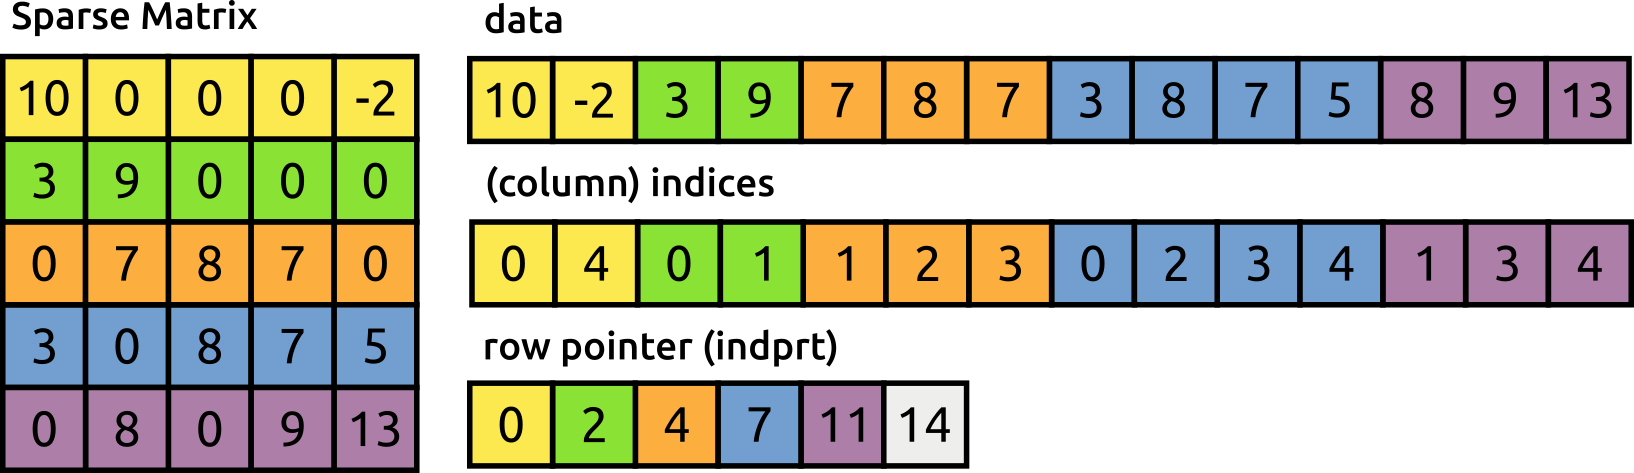
\includegraphics[width=0.7\linewidth]{media/csr-matrix}
	\caption{Beispiel CSR Matrix}
	\label{fig:csr-matrix}
\end{figure}
~\\~\\
Können wir die \textbf{Matrix-Dimension} aus diesem Format ablesen?
\begin{itemize}
	\item Zeilendimension: $m = \texttt{len(indptr)} - 1$
	\item Spaltendimension?\\
			Man könnte vermuten $n=\texttt{max(indices)}$, aber was ist wenn die letzte Spalte der Matrix eine Nullspalte ist?\\
			Stattdessen könnte man in \texttt{indptr}[0] die Spaltendimension speichern, da das erste Adjazenzpaar immer mit dem Index \texttt{0} beginnt.
\end{itemize}
~\\
Wann sparen wir \textbf{Speicherplatz}?\\
Wir definieren $$\texttt{nnz} := \texttt{len(data)} = \text{Anzahl der Nichtnulleinträge}.$$
Dann muss in den entsprechenden Formaten folgende Anzahl an Zahlen gespeichert werden:
\begin{itemize}
	\item Dense: $m\cdot n$
	\item CSR: $2 \cdot \texttt{nnz} + (m+1)$
\end{itemize}
Und daher
$$2 \cdot \texttt{nnz} + (m+1) < m\cdot n ~~~\Leftrightarrow~~~ \texttt{nnz} < \frac{(n-1)m - 1}{2}$$
~\\~\\
\textbf{Beispiel:} Tridiagonalmatrix\\~
[Tafel: Grafik zu Tridiagonalmatrix]
\begin{itemize}
	\item Dense: $n^2$
	\item Nichtnulleinträge: $\texttt{nnz} = n + 2 (n-1) = 3n -1$
	\item CSR: $2 \cdot \texttt{nnz} + (m+1) = 2 (n + 2 (n-1)) + n+1 = \ldots = 7n -3$ ~~((affin) linear in $n$)
\end{itemize}
[Tafel: Grafik $n^2$ VS $7n -3$]
\subsubsection{Sonstiges}
\textbf{Andere Formate}
\begin{itemize}
	\item \textbf{Compressed Sparse Column (CSC)}\\
	Während CSR effizientes \textit{row slicing} (man kann schnell die $i$-te Zeile berechnen; daher effizient: $x \mapsto A\cdot x$) ermöglicht, so ermöglicht CSC effizientes \textit{column slicing} (daher effizient: $x \mapsto x^\top A = (A^\top x)^\top$).\\
	Sowohl CSR als auch CSC eignen sich nicht gut zur inkrementellen Manipulation/Erzeugung einer Matrix.
	\item \textbf{Coordinate list (COO)}\\
	Speichert die Listen \texttt{(row, column, value)}\\
	Zum Beispiel: Rating-Daten (Benutzer, Produkt (wie Film), Bewertung)
\end{itemize}
~\\
Die entsprechende Bibliothek in Python ist \textbf{\texttt{scipy.sparse}}\\
\url{https://docs.scipy.org/doc/scipy/reference/sparse.html}

%%%%%%%%%%%%%%%%%%%%

\subsection{Anwendung: PageRank}
\textbf{An Application of Eigenvectors: The \textit{PageRank}}

\textbf{Aim:} To rank results of a web search engine (such as Google) according to the \textit{``importance''} of the web pages.\\

\textbf{1998:} For this purpose, Larry Page and Sergei Brin developed the PageRank algorithm as the basis of the
Google empire.\\

\textbf{Assumption:} \textit{``important''} means more links from other (important) web pages.\\


\textbf{ Idea:}
Let us think of the web as a directed graph, i.e., web pages are nodes and links from one page to another, i.e, from one node to another, are modeled as directed edges. For example a web structure consisting of 11 web pages could look as follows:
\begin{center}
	\begin{minipage}[c]{0.5\textwidth}
		%	Potential Web Structure:
		\begin{tikzpicture}[->,>=stealth',shorten >=1pt,auto,node distance=1.9cm,	semithick]
		\tikzstyle{every state}=[fill=red,draw=none,text=white]
		\node[state,fill=blue] (A)                   {$1$};
		\node[state,scale=2.2] (B)    [right of=A]               {$2$};
		\node[state,fill=yellow,scale=1.8] (C)    [right of=B]    {\color{black}$3$};
		\node[state,fill=green] (D)    [below of=A]               {\color{black}$4$};
		\node[state,fill=brown] (E)    [below left of =C]               {$5$};
		\node[state,fill=green] (F)    [below of=C]               {\color{black}$6$};
		\node[state,fill=purple,scale=0.7] (G)    [below of=D]               {$7$};
		\node[state,fill=purple,scale=0.7] (H)    [right of=G]               {$8$};
		\node[state,fill=purple,scale=0.7] (I)    [right of=H]               {$9$};
		\node[state,fill=purple,scale=0.7] (J)    [right of=I]               {$10$};
		\node[state,fill=purple,scale=0.7] (K)    [right of=J]               {$11$};
		\path (B) edge [bend left=15pt]  (C)
		(C) edge [bend left=15pt]  (B);
		\path (D) edge   (A)
		(D) edge   (B);
		\path (E) edge   (D)
		(E) edge (B);
		\path (F) edge [bend left=20pt]  (E)
		(E) edge [bend left]  (F)
		(E) edge  (B);
		\path (G) edge   (B)
		(G) edge [bend left=5pt] (E);
		\path (H) edge   (B)
		(H) edge (E);
		\path (I) edge   (B)
		(I) edge [bend right=5pt](E);
		\path (J) edge [bend right=5pt](E);
		\path (K) edge [bend left=2pt](E);
		\end{tikzpicture}

	\end{minipage}
\end{center}

We now randomly place a random surfer according to the initial probability distribution $x^0 = (x^0_1, \ldots, x_n^0)$ on this graph. Here, $n$ (in the example above $n=11$) denotes the number of web pages and $x^0_i$ denotes the probability that the random surfer \textit{starts} at web page $i$. Further let $e := (1,\ldots,1)^T$, then the fact that $x^0$ is a probability distribution (i.e., probabilities sum up to $1$) translates into $e^Tx^0 =x^0_1+\ldots+x_n^0 =1$. Now we make the assumption that the random surfer moves...
\begin{itemize}
	\item[(1)] ...with probability $\alpha \in (0,1)$ according to the link structure (with equal preferences to outgoing links)
	\item[(2)] ...with probability $(1-\alpha)$ he can teleport to a random page (with equal probability) to prevent stranding in deadlocks
	\item[$\rightarrow$] Pages, where the random surfer is more likely to appear in the long run based on the web's structure are considered more important.
\end{itemize}

These two movements can be described by multiplying the current probability distribution with the two following matrices:
$$P_1={
	\left(  \begin{tabular}{cccccccccccc}
	~ & 1    & 2   & 3    & 4    & 5    & 6 & 7     & 8   & 9  & 10   & 11    \\
	1 & 1    &~     &  ~   & 1/2  &    ~ & ~ & ~     &  ~  &  ~   & ~ &    ~  \\
	2 & ~    & ~    &  1   & 1/2  & 1/3  &   & 1/2   & 1/2 & 1/2 &   &    \\
	3 & ~    & 1    &  ~   &      &      &   &       &     &     &   &    \\
	4 & ~    &  ~   & ~    &      &  1/3 &   &       &     &     &   &  \\
	5 & ~    &  ~   & ~    &      &      & 1 & 1/2   & 1/2 & 1/2 & 1 & 1 \\
	6 & ~    &  ~   &  ~   &      & 1/3  &   &       &     &     &   &  \\
	7 & ~    & ~    &  ~   &      &      &   &       &     &     &   &  \\
	8 &~     & ~    &  ~   &      &      &   &       &     &     &   &  \\
	9 & ~    &  ~   &  ~   &      &      &   &       &     &     &   &  \\
	10 & ~    &  ~   & ~    &      &      &   &       &     &     &   &  \\
	11 & ~    &  ~   & ~    &      &      &   &       &     &     &   &
	\end{tabular} \right)
},
~~~~P_2 := \frac{1}{n}ee^T= \left(\frac{1}{n}\right)_{ij}$$
More precisely,
\begin{itemize}
	\item[(1)] \textbf{Link structure:} $P_1$ is the probability matrix (column stochastic) defined by\\
	$P_1^{ij}:=$  Probability that random surfer moves from page $j$ to page $i$ defined by the link structure
	\item[(2)] \textbf{Jumps:}  $P_2$ is the probability matrix (column stochastic) defined by\\
	$P_2^{ij} := \frac{1}{n}$= Probability that random surfer jumps from page $j$ to page $i$
\end{itemize}
The movement of the random surfer is then completely defined by the probability matrix
$$P = \alpha P_1 + (1-\alpha)P_2 .$$
This matrix is also known as the \textit{\textbf{Google Matrix}}. For the next time instances we therefore obtain
\begin{align*}
x^1 &=  \alpha P_1 x^0 + (1-\alpha) P_2 x^0 = Px^0  \\
x^2 &=  \alpha P_1 x^1 + (1-\alpha) P_2 x^1 = Px^1 \\[0.1cm]
x^{k+1} &=  \alpha P_1 x^k + (1-\alpha) P_2 x^k = Px^k = P^{k+1}x^0 \\[0.1cm]
x^* &=  \lim_{k\to \infty} x^k =: \textbf{\textit{PageRank}}
\end{align*}
\textbf{Observations:}
\begin{itemize}
	\item One can easily show that $P_1$, $P_2$ and thus $P$ are column stochastic (i.e., $e^TP = e^T$)
	\item Consequently, since $x^0$ is a probability distribution (i.e., $e^Tx^0 = 1$), also $e^Tx^k = 1$ for all $k$ and $e^Tx^*=1$
\end{itemize}

\textbf{Question:} \\
Does this sequence $\{x^k\}_{k \in \mathbb{N}}$ of vectors converge (to a steady state)? More precisely, is there a $x^* = \lim_{k\to \infty} x^k= \lim_{k\to \infty} P^kx^0$, so that
\begin{equation} \label{eq:PageRank_eigprob}
Px^* = 1 x^* .
\end{equation}
\begin{itemize}
	\item[$\rightarrow$] With other words, is there an \textit{\textbf{eigenvector}} $x^*$ to the \textit{\textbf{eigenvalue}} $1$ of the matrix $P$?
	\item[$\rightarrow$]\textit{\textbf{Eigenvalue algorithms}} are developed to solve such problems. One of them is the \textit{\textbf{Power iteration}}, which, applied to the eigenvalue problem above, produces precisely the sequence
	$$x^k = P^k x^0.$$
\end{itemize}
Intuitively, in the limit most of the ``mass'' would be located at web pages that have many incoming links and would therefore be ranked as being more important. In fact, the $i$-th component of $x^*$ is called the \textit{PageRank} of the web page $i$.\\~\\
Remark: \textit{Perron Theorem}\\
A positive damping factor $\alpha>0$ is also technically necessary as it assures that the matrix $P$ has only strictly positive coefficients. The Perron Theorem then sates that its largest eigenvalue is strictly larger than all other eigenvalues (in magnitude). Thus the convergence of the Power method is guaranteed. Since the matrix is column stochastic one can further show that the largest eigenvalue is $1$.

\subsubsection{Compute Page Rank matrix}
\url{https://de.wikipedia.org/wiki/Google-Matrix}\\
adjazenz matrix, normalize, dangling nodes,..

\subsubsection{Implementation Issues}
How to implement $P_2 x$?

\newpage
\subsection{Anwendung: Optimierung}
	Let $A \in \mathbb{R}^{n \times n}$ be symmetric and positive definite (spd). Then $A$ is in particular invertible, so that the
linear system
$Ax = b$
has a unique solution $x^* \in \mathbb{R}^{n}$  for all $b \in \mathbb{R}^{n}$  . Let us relate this linear system to an optimization problem.
For this purpose we define for a fixed spd matrix $A$ and fixed right-hand side $b$ the function
$$f:=f_{A,b} : \mathbb{R}^{n}  \to \mathbb{R}, ~~x  \mapsto \tfrac{1}{2} x^T Ax - b^T x.$$
Then one can show the equivalence
$$Ax^* = b ~~~\iff~~~	x^* = \arg \min_{x\in\mathbb{R}^{n}} f (x).	$$
In words, $x^*$ solves the linear system on the left-hand side if and only if $x^*$ is the unique minimizer of the
functional $f$. In fact, you will learn in the next semester that the condition $Ax^* = b$ is the necessary first-order optimality
condition:
$$0 = \nabla f (x) = Ax - b.$$
Due to the convexity of $f$ this condition is also sufficient.
%	The vector $\nabla f (x)$ is called the gradient of $f$ at $x$ and can be considered the first-order derivative of $f$ (if $n = 1$, then this is precisely $f' (x)$ which we know from high school).
Consequently, solving linear systems which involve spd matrices is equivalent to solving the associated
optimization problem above, i.e., minimizing the function $f (x) = \tfrac{1}{2} x^T Ax - b^T x$. Thus, in this context iterative methods
for linear systems, such as the Richardson iteration, can also be interpreted as optimization algorithms.
Let us consider the (relaxed) Richardson iteration for $Ax = b$, i.e.,
$x_{k+1} = (I - \theta A)x_{k} + \theta b$.
After some minor manipulations and making use of $\nabla f (x_{k} ) = Ax_{k} - b$ we arrive at the equivalent
formulation
$$x_{k+1} = x_{k} - \theta\nabla f (x_{k} ).$$
The latter is what is called a gradient method. A step from $x_{k}$ into (an appropriately scaled) direction of the gradient
$\nabla f (x_{k} )$ yields a decrease in the objective function $f$ , i.e., $f (x_{k+1} ) \leq  f (x_{k}$ ). Along the Richardson aka Gradient method the scaling (also called step size) $\theta$ is fixed (in a machine learning context the step size $\theta$ is called the \textit{learning rate}). However, one could also choose a different
$\theta_k$  in each iteration step. This gives the more general version
\begin{equation}\label{steepest_descent_method}
	x_{k+1} = x_{k} - \theta_k  \nabla f (x_{k} ).
\end{equation}
The well known method of \textit{steepest descent} is given by choosing
\begin{equation} \label{steepest_descent_stepsize}
	\theta_k  = \frac{r_k^\top r_k}{ r_k^\top   Ar_k  },
\end{equation}
where $r_k : = Ax_{k} - b$ is the $k$-th residual. This choice can be shown to be optimal in terms of convergence
speed. Even more general, one can think of using a different preconditioner $N_k$ in each iteration step
$$x_{k+1} = x_{k} - N_k \nabla f (x_{k} ),$$ 
i.e., representing the gradient with respect to another inner product. This will later correspond to Newton-type optimization algorithms.
%%%%%%%%%%%%%%%%%%%%
%%%%%%%%%%%%%%%%%%%%
\clearpage
\section{Projektaufbau planen}
\begin{figure}[h!]
	\centering
	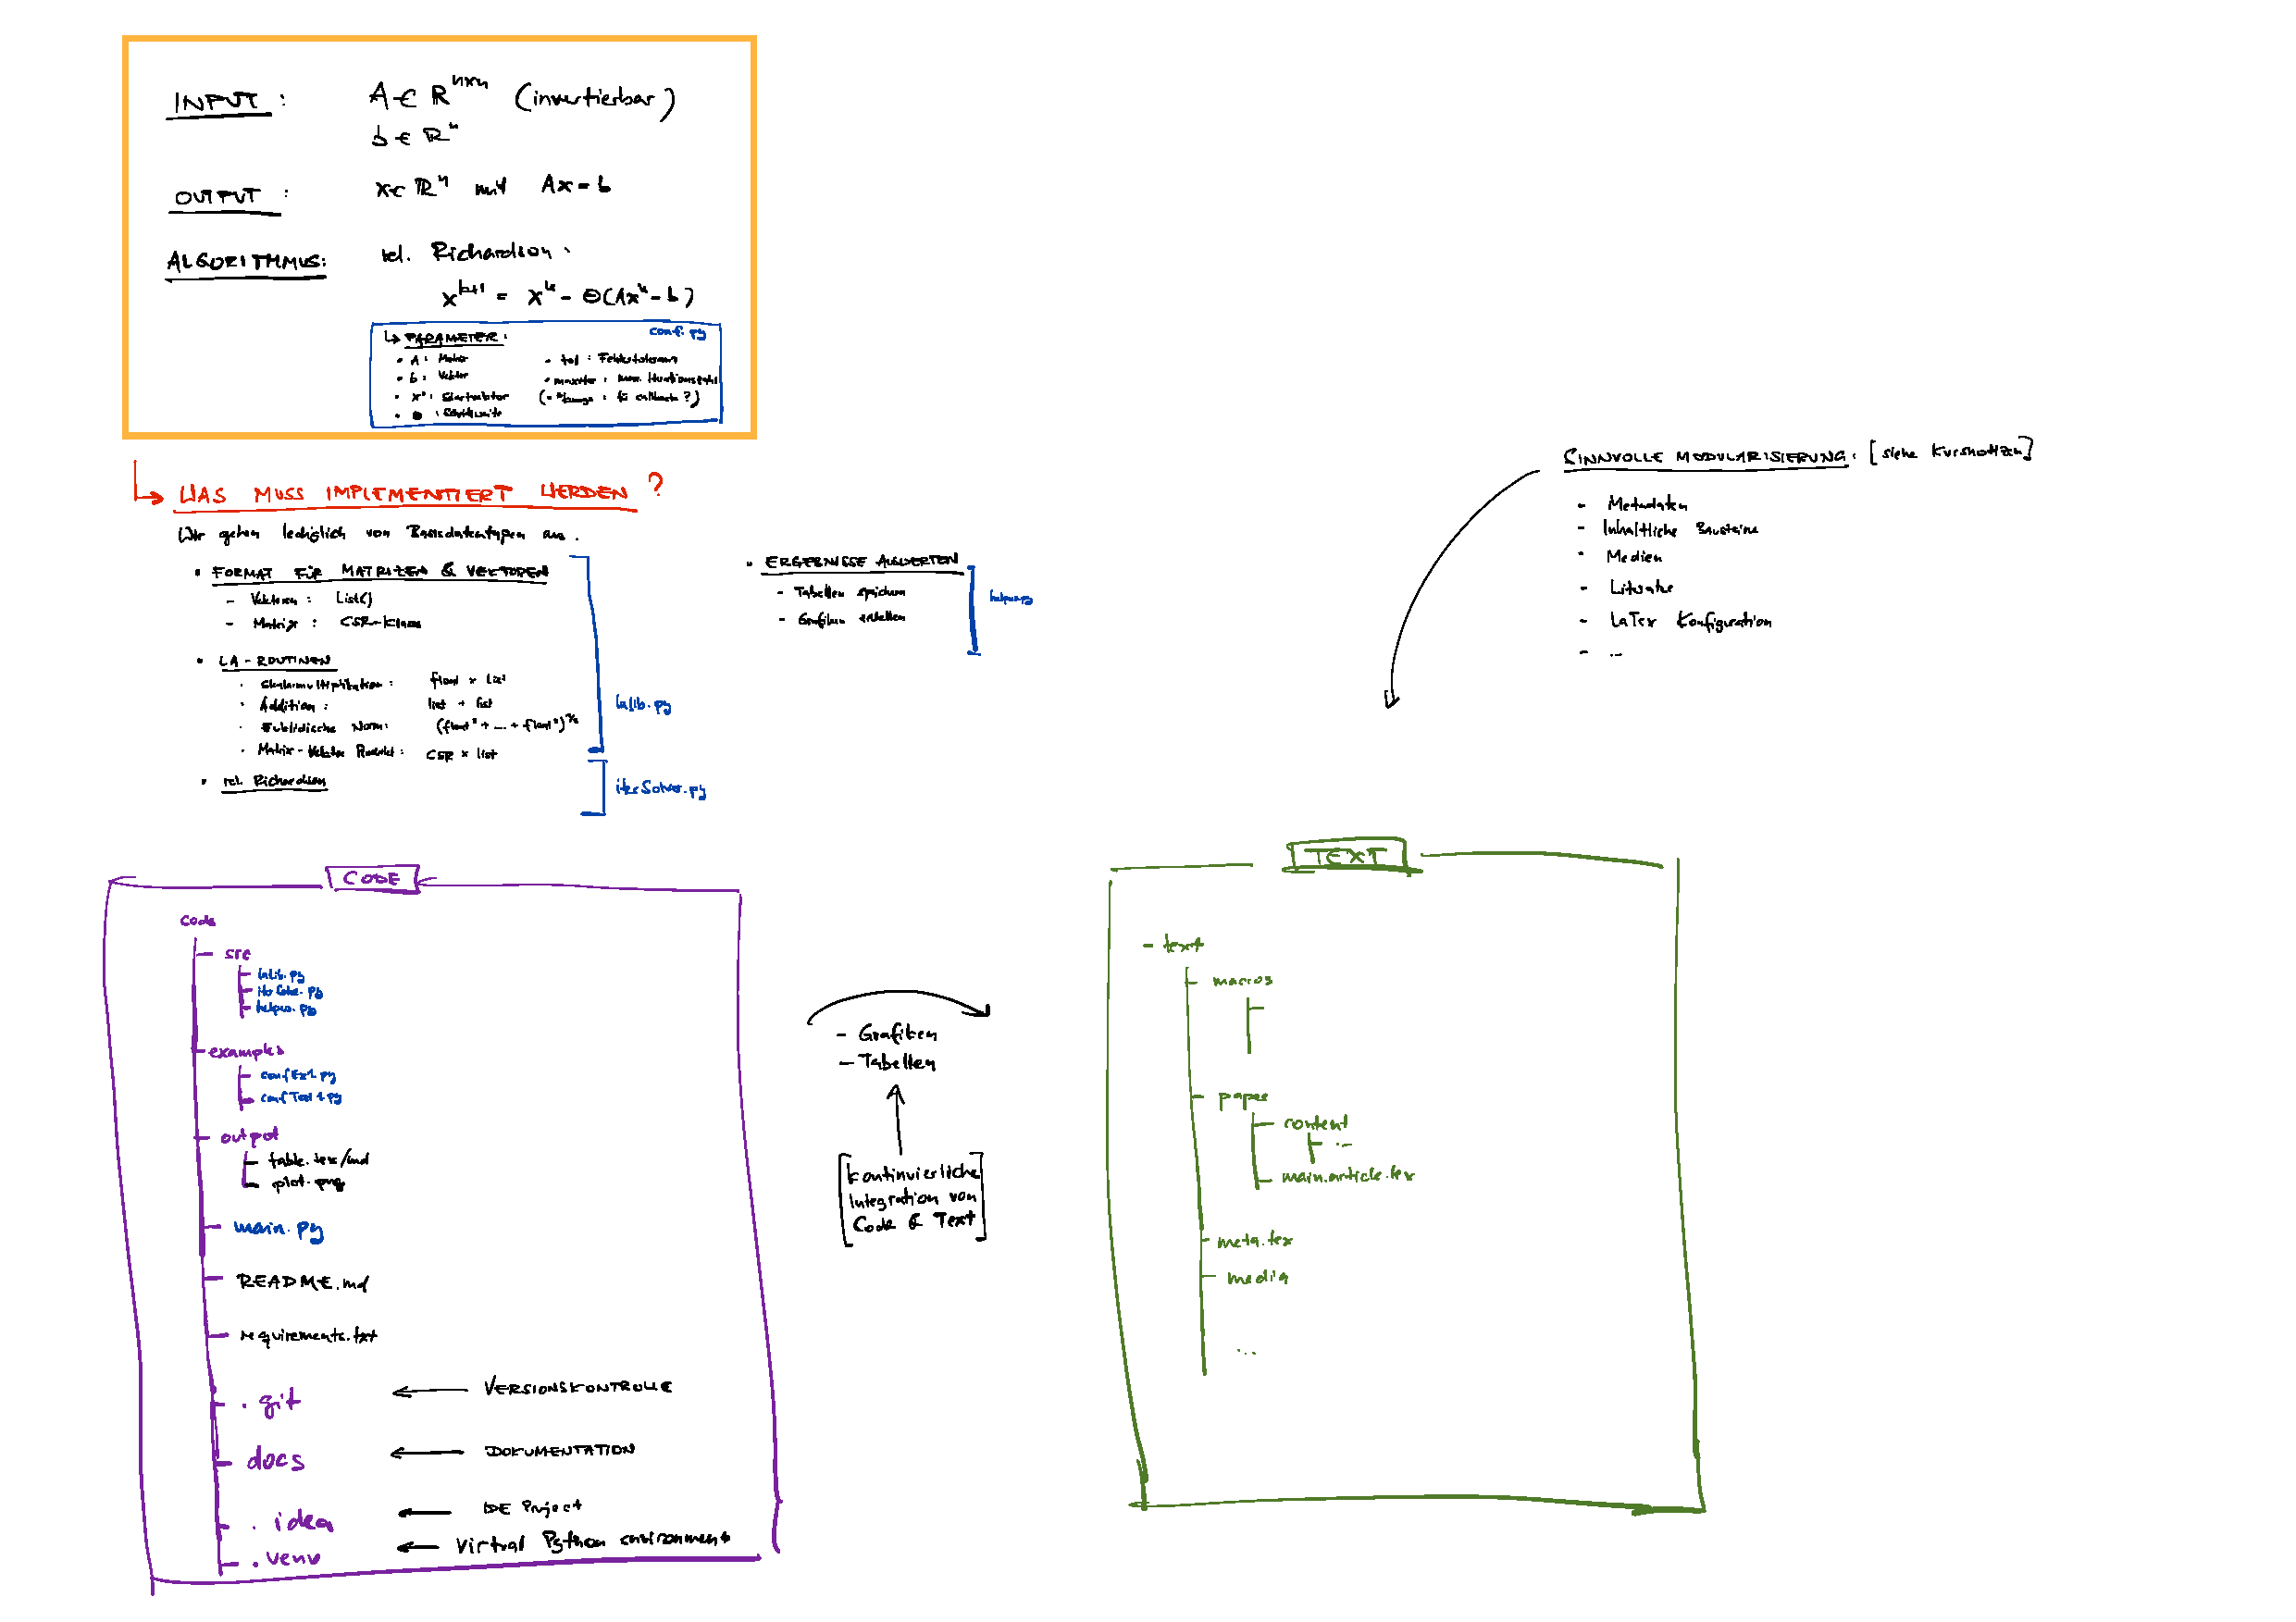
\includegraphics[width=1.3
	\linewidth]{./media//ProjectMindMap2}
	\caption[Mindmap zum Projektaufbau]{Skizze zu einem möglichen Projektaufbau.}
	\label{fig:projektaufbau}
\end{figure}
~\\~\\
\textbf{Fallbeispiel:} Sie müssen eine mathematische Arbeit über ein numerisches Thema verfassen (z.B. im Rahmen eines Seminars oder der Bachelor- bzw. Masterarbeit).
%{\beispiel \textbf{Beispielthema:} Iterative Löser (genauer Splitting-Verfahren) für lineare Gleichungssysteme
%$$Ax = b, $$
%wobei $A\in\Rnn$ und $b\in \Rn$ gegeben sind und wir eine Lösung $x \in \Rn$ suchen. Splitting-Verfahren generieren eine Fixpunktiteration
%$$x_{k+1} = Mx_k + Nb, ~x^0\in\Rn,$$
%sodass $x_k  \to x$ für $k \to \infty$. Unterschiedliche Wahl von $M$ und $N$ liefert unterschiedliche Verfahren.}
%~\\

\subsection{Code}
Nachdem Sie die Fragestellung verstanden haben, versuchen Sie zunächst einmal numerische Ergebnisse zu produzieren. Dazu überlegen Sie sich idealerweise eine vernünftige Code-Infrastruktur, z.B.:

%CODE
\begin{itemize}
	%
	\item Programmiersprache (hier Python)
	%
	\item Arbeitsumgebung: jupyter, IDE wie Spyder, Texteditor+Konsole (hier IDE \pycharm)
	%
	\item Versionskontrolle und backup\\
	{\beispiel \texttt{git, github, (seafile?)}}
	%
	\item Was ist der Input? Hyperparameter? Welches Format? (Zahlen, Matrizen, Text, Grafik,...)\\
	{\beispiel Matrizen/Vektoren $A$, $b$, Verfahren?, maximale Iterationszahl, Fehlertoleranz,...}
	%
	\item Was ist der Output? Welches Format? (Zahlen, Matrizen, Text, Grafik, Tabelle,...)
	\\
	{\beispiel Vektoren $x$, Grafiken und Tabellen die den Konvergenzverlauf zeigen,...}
	%
	\item Was ist die Kernaufgabe des Codes? Welche Funktionen können modularisiert werden ? (linalg, src, helpers,...)\\
	{\beispiel Verschiedene Funktionen für: Iteration, Erzeugung und speichern von Grafiken und Tabellen,... }
	%
	\item Was sind variable Parameter, die man ggf. komfortable in einer zentralen Konfigurationsdatei ändern möchte (conf.py)? \\
	{\beispiel Beispiel: Problem $A, b$, Maximale Iterationsanzahl, Fehlertoleranz,...}
	%
	\item Was sind die Anforderungen an die Python-Umgebung? Werden externe Pakete benötigt?\\ \texttt{requirements.txt}\\
	{\beispiel \texttt{matplotlib} zur Erstellung von Grafiken,...}
	%
	\item Sie schreiben Tests, welche der Code mindestens bestehen muss.\\ \texttt{pytest, unittests}\\
	{\beispiel Sie testen ihren Löser auf verschiedenen Beispielen $(A,b;x)$, bei denen Sie die Lösung $x =A^{-1}b$ kennen oder diese gar nicht existiert.}
	%
	\item Dokumentation und clean Code\\
	{\beispiel PEP 8, \texttt{sphinx},...}
\end{itemize}
Wenn Ihr Betreuer in der Besprechung nach anderen Beispielen verlangt, können Sie diese nun bequem über Ihre Konfigurationsschnittstelle einspeisen.

%\subsubsection{Katastrophen vermeiden}
%\textbf{Szenario 1}\\
%Stellen Sie sich vor die Platte Ihres Rechners versagt kurz vor Abgabe der Abschlussarbeit und Ihre Daten sind ganz oder teilweise verloren, da Sie diese gar nicht oder nur sporadisch/manuell auf einem anderen Medium (z.B. externe Festplatte oder USB-Stick) abgesichert haben. Damit Sie von diesem Szenario verschont bleiben, synchronsieren Sie gleich Ihre Daten automatisiert (d.h. mithilfe eines geeigneten Client/Software) in einer Cloud (zentraler Dateispeicher). Mit Ihrer ZIMK-Kennung stehen Ihnen 16GB Speicherplatz auf dem \seafile-Server des Landes Rheinland-Pfalz in Mainz zu Verfügung. Damit sind Ihren Daten nicht nur abgesichert, sondern stehen auch auf sämtlichen Endgeräten redundant zur Verfügung.\\
%~\\
%\textbf{Szenario 2}\\
%Nun stellen Sie sich vor, Ihr Betreuer verlangt nach einer (vermeintlich leichten) Modifikation Ihres Codes, {\beispiel zum Beispiel einer Schrittweitensteuerung}. Bei der Implementierung dieser Modifikation  ``zerschießen'' Sie allerdings Ihren Code und die ursprüngliche Funktionalität ist nicht mehr gegeben. Nun haben Sie zwar Ihre Daten hochverfügbar in der Cloud (welche mitunter Backups zu festen Zeiten anlegt), aber Sie haben (noch) nicht die Möglichkeit zu einer bestimmten von Ihnen fest eingeloggten Code-Version zurückzukehren. Damit Sie von diesem Szenario verschont bleiben, nutzen Sie gleich das Tool/Anwendungssoftware \git~, welches eine automatisierte Versionskontrolle ermöglicht. Die Uni Trier stellt in diesem Rahmen einen \gitlab~Server zur Verfügung.\\
%~\\
%\textbf{Szenario 3}\\
%Nun stellen Sie sich vor, Sie haben zwei Wochen (oder Tage) nicht mehr an Ihrem Code gearbeitet und Sie müssen sich stark anstrengen, um Ihren Code nochmal selber zu durchblicken. Oder Ihr Betreuer möchte aufbauend auf Ihrem Code weitere Arbeiten vergeben oder diesen gar selbst nutzen. Wenn man nicht selbst der Entwickler ist, hat man in der Regel schlechte Chancen einen fremden Code (in angemessener Zeit) zu verstehen und zu benutzen.  Damit Ihr zukünftiges Ich oder andere von diesem Szenario verschont bleiben, dokumentieren Sie gleich zu Beginn fein säuberlich Ihren Code. Dazu werden wir geeignete Tools kennenlernen.\\
~\\
Insgesamt erhalten Sie möglicherweise eine Verzeichnisstruktur wie in Abb. \ref{fig:vz-struktur-code} für Ihren Projektblock \textbf{``Code''}.\\
\begin{figure}[h!]
	\centering
%	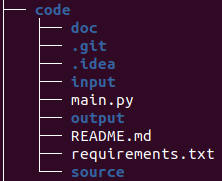
\includegraphics[width=0.2\linewidth]{\PathToMedia/progprak/vz-struktur-code}
%	~\\
\begin{minipage}{0.4\textwidth}
\begin{verbatim}
|-- code
    |-- docs
    |-- src
    |   |-- linalg.py
    |   |-- iterative_solver.py
    |   |-- utils.py
    |-- examples
    |   |-- example_pagerank.py
    |   |-- example_heatequation.py
    |   |-- ...
    |-- data
    |-- test
    |-- main.py
    |-- README.rst
    |-- LICENSE
    |-- requirements.txt
    |-- .git
    |-- .idea
\end{verbatim}
\end{minipage}
	\caption[Beispiel: Verzeichnisstruktur für \texttt{code}]{Eine mögliche Verzeichnisstruktur für das Code-Projekt. Beachten Sie, dass \texttt{requirements.txt, .git} und \texttt{.idea} automatisch erzeugt werden.}
	\label{fig:vz-struktur-code}
\end{figure}

\subsection{Text (skip)}
Sie haben bereits erste numerische Ergebnisse produziert, die Sie Ihrem Betreuer oder der Welt in einem schönen Text präsentieren möchten. Als Mathematiker werden Sie feststellen, dass Sie unter Verwendung von Microsoft Office oder LibreOffice schnell an den Rande des Wahnsinns getrieben werden: Sie müssen mathematische Formeln bequem schreiben können, Nummerierungen sollten automatisch erzeugt werden, Grafiken und Tabellen sollten über generische Pfade importiert werden (ggf. gesteuert über Bash-Skripte), Sie brauchen ein Literaturverzeichnis etc. Spätestens ab diesem Punkt kommt \TeX~ bzw. \LaTeX~ins Spiel, das nach einer kleinen Einarbeitungsphase Ihr Leben als Textautor nachhaltig vereinfachen wird.\\
~\\
Stellen Sie sich \LaTeX~wie eine Programmiersprache vor: Auch hier gilt es Ihr (Text-)Projekt in geeignete Module zu unterteilen. Das dient nicht nur zur besseren Übersicht, sondern auch zur Wiederverwendbarkeit bestimmter Bausteine für andere Projekte (z.B. Bachelorarbeit $\to$ Masterarbeit). Eine Modularisierung könnte wie folgt aussehen:
\begin{itemize}
	\item Inhaltliche Bausteine: Zusammenfassung, Kapitel 1, Kapitel 2, Listings,...
	\item Medien: Bilder, pdfs,...
	\item Literatur: pdfs, Literaturverzeichnis \texttt{literature.bib},...
	\item Metadaten: Autorname, Titel, Datum,...
	\item \LaTeX~Spezifizierung: usepackages, commands, style,...
\end{itemize}
Insgesamt erhalten Sie möglicherweise eine Verzeichnisstruktur wie in Abb. \ref{fig:vz-struktur-text} für Ihren Projektblock \textbf{``Text''}.\\
\begin{figure}[h!]
	\centering
\begin{minipage}{0.4\textwidth}
\begin{verbatim}
|-- text/
    |-- src/
    |   |-- macros/
    |   |   |-- meta.tex
    |   |   |-- usepackages.tex
    |   |   |-- style.tex
    |   |   |-- commands.tex
    |   |   |-- ...
    |   |-- content/
    |   |   |-- abstract.tex
    |   |   |-- introduction.tex
    |   |   |-- section1.tex
    |   |   |-- section2.tex
    |   |   |-- listing.py
    |   |   |-- ...
    |-- media/
    |   |-- picture.png
    |   |-- picture.jpg
    |   |-- ...
    |-- literature/
    |   |-- literature.bib
    |   |-- pdfs/
    |   |   |-- book.pdf
    |   |   |-- paper.pdf
    |   |   |-- ...
    |-- main.tex
\end{verbatim}
%    |-- talk/
%    |   |-- main.beamer.tex
\end{minipage}
	\caption[Beispiel: Verzeichnisstruktur für \texttt{text}]{Eine mögliche Verzeichnisstruktur für das Text-Projekt.}
	\label{fig:vz-struktur-text}
\end{figure}
%~\\
%\subsection{Effizient arbeiten: Kontinuierliche Integration von Code und Text.} In regelmäßigen Treffen präsentieren Sie Ihrem Betreuer die bisherigen Ergebnisse. Sie kommen nicht selten zu dem Entschluss weitere Tests zu verschiedenen Input-Parametern durchzuführen. Dabei ändern sich selbstverständlich die Output-Werte inkl. Grafiken und Tabellen, die Sie zuvor müßselig in Ihr \LaTeX~Dokument integriert haben. Um diese Integration gleich automatisiert ablaufen zu lassen, verwenden Sie eine geeignete Verzeichnis-Struktur für Ihr Gesamtprojekt, generische Pfade (Variablen) und geeignete Tools, um bequem Code und Text dynamisch zu verheiraten.\\




%{\color{red} $\rightarrow$ Alles in allem erhalten Sie beispielsweise eine Verzeichnisstruktur wie in Abb. \ref{fig:vz-struktur} für Ihr Gesamtprojekt.}\\
%\begin{figure}[h!]
%	\centering
%	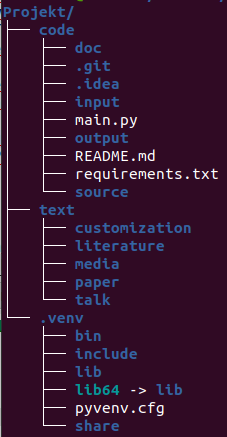
\includegraphics[width=0.2\linewidth]{\PathToMedia/progprak/vz-struktur}
%	\caption[Verzeichnisstruktur für \texttt{code}]{So könnte Ihre Verzeichnisstruktur für das Gesamtprojekt aussehen.}
%	\label{fig:vz-struktur}
%\end{figure}
%
